\section{Discussion}

\subsubsection{Correspondence search}
KLT vs Harris matching

\subsubsection{Bundle Adjust}
While the approach described in \cref{ba_cont} was implemented the results did not meet our expectations. Even after thorowly evaluating and improving the code for dozens of hours no satisfying results were obtained with bundle adjustment enabled.

The plots in \cref{fig:ba_comp} show, that the reprojected landmarks and keypoints before and after bundle adjustment match correctly. Further testing showed that the keypoints are also tracked correctly accros the frames. 
The various parameters such as the number of fixed frames, sliding window and the bundle adjustment frequency were tested accros the board. The results were always worse than without bundle adjustment however.
One example of strangely optimized landmarks is shown in \cref{ba_vs_wo_ba}. The landmarks all correlated into a line such that the trajectory fails.

Since this bug messed up the bundle adjustment, all datasets and results are with bundle adjustment deactivated.

\begin{figure}
	\centering
	\includegraphics[width=0.8\textwidth]{cont/ba_comp}
	\caption{Reprojected landmarks and corresponding keypoints before and after bundle adjustment.}
	\label{fig:ba_comp}
\end{figure}


\begin{figure}
\centering
   \begin{subfigure}[b]{0.55\textwidth}
   \includegraphics[width=1\linewidth]{cont/wo_ba}
\end{subfigure}

\begin{subfigure}[b]{0.55\textwidth}
   \includegraphics[width=1\linewidth]{cont/w_ba}
   \label{ba_vs_wo_ba}
\end{subfigure}
\caption{Bundle adjusted landmarks correlate in a line.}
\end{figure}
\end{document}



\subsubsection{Pose estimation algorithm}
We investigated pose estimation with DLT refinement after the P3P-Guess and without refinement (using the last P3P guess from RANSAC). It turned out, that very often the P3P-guess was a lot better and especially more robust then the DLT refinement. \cref{parking_result_fig_dlt} shows the estimated trajectory with DLT refinement. It is clearly worse then the P3P estimate as shown in \cref{parking_result_fig}. That's why we used the last P3P guess in our implementation.
\begin{figure*}[ht!]
    \centering
    \begin{subfigure}[t]{0.5\textwidth}
        \centering
        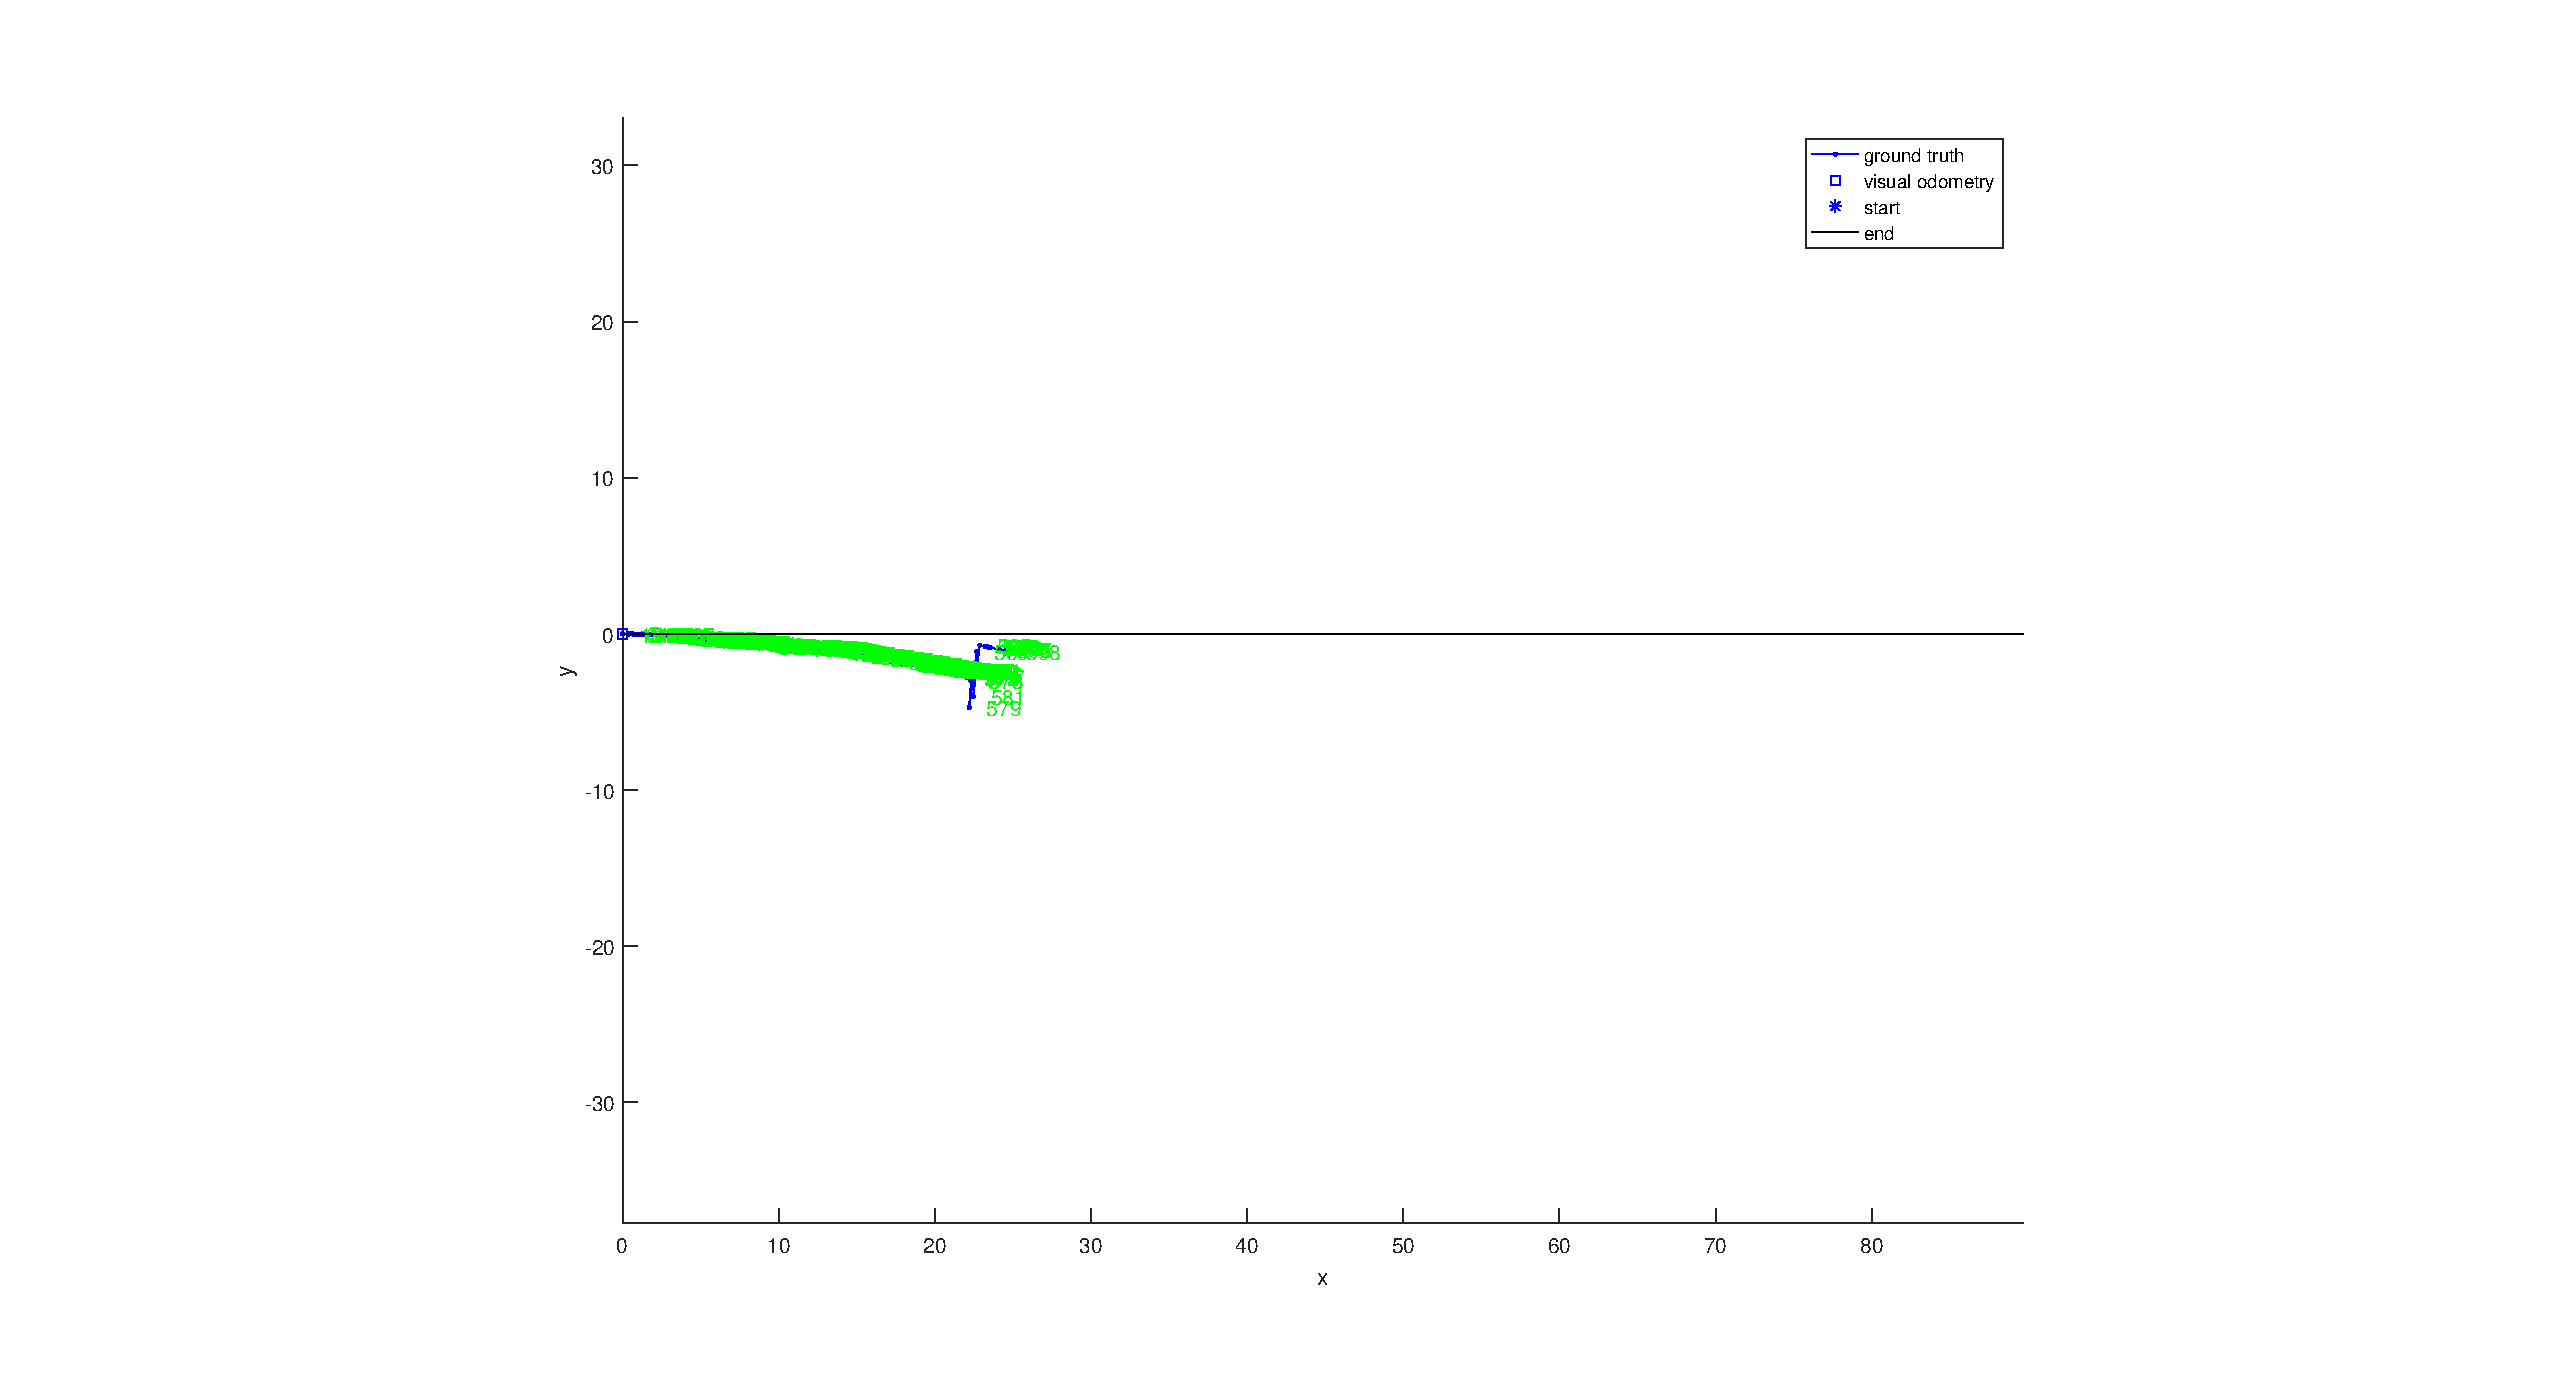
\includegraphics[height=2.7in]{results/trajectory_parking_dlt.eps} 
        \caption{Trajectory vs. ground truth}
    \end{subfigure} 
    \begin{subfigure}[t]{0.5\textwidth}
        \centering
        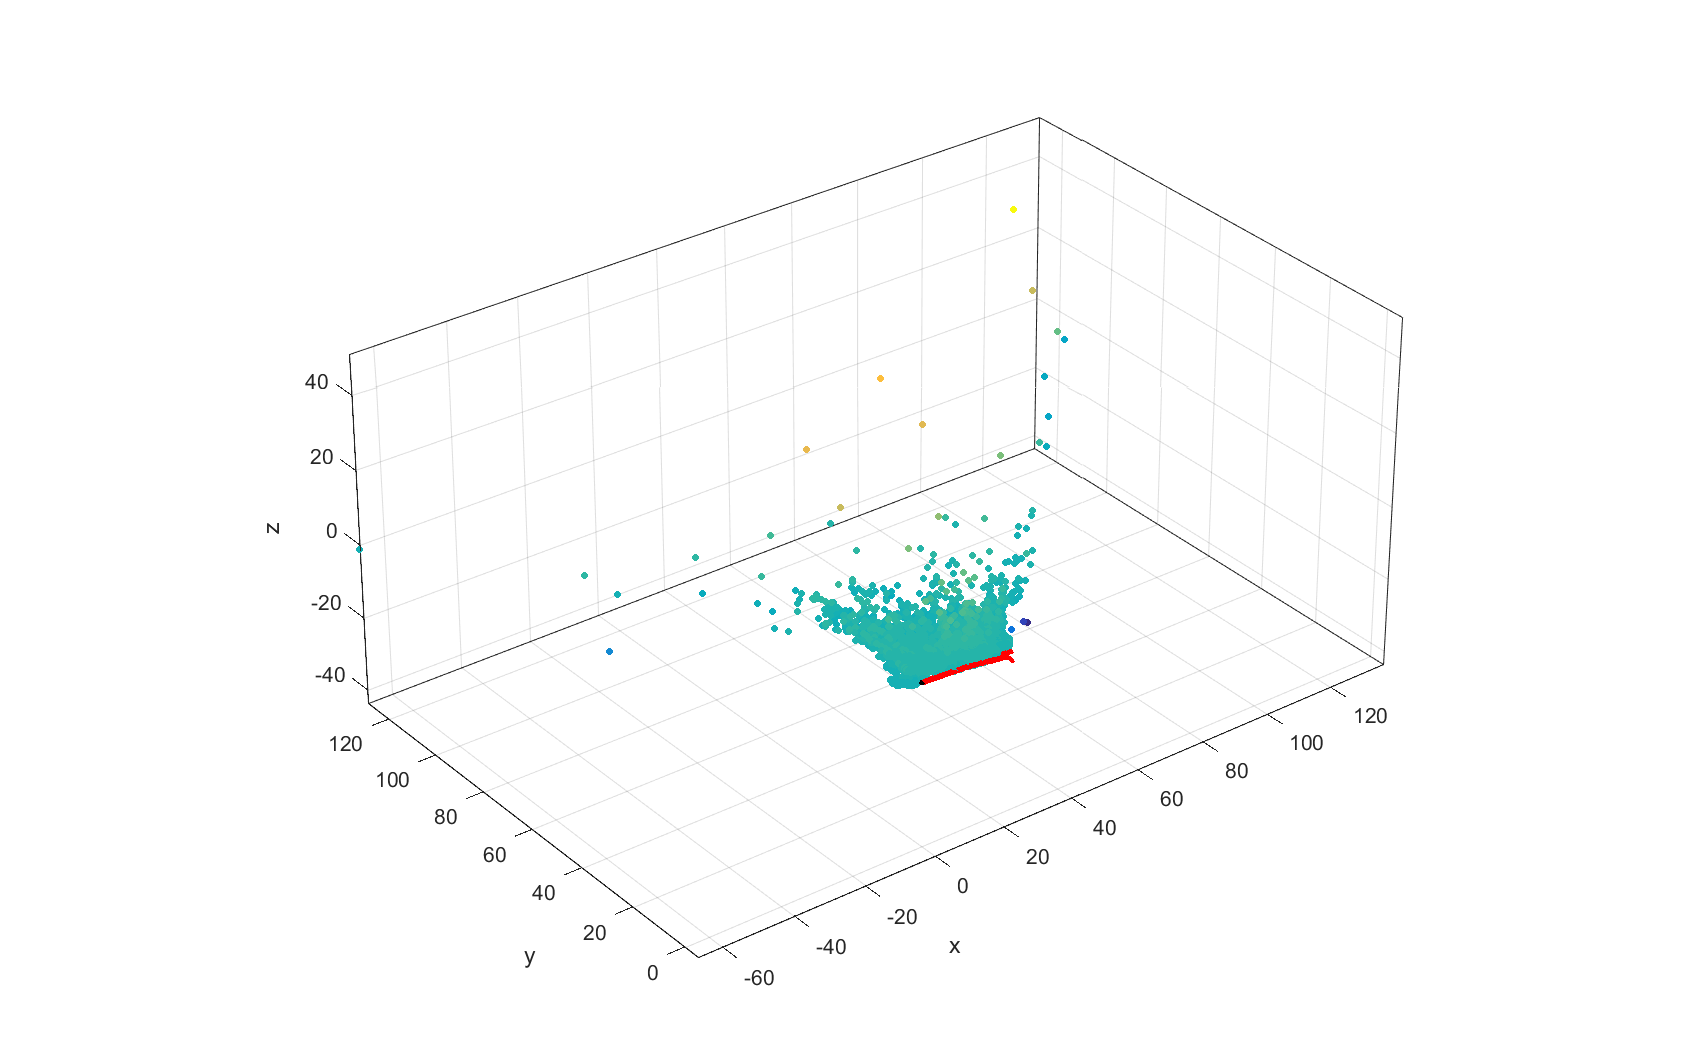
\includegraphics[height=2.7in]{results/landmarks_parking_dlt.eps}
        \caption{3D landmarks}
    \end{subfigure}
    \caption{Parking Dataset Results with DLT refinement}
		\label{parking_result_fig_dlt}
\end{figure*}

\subsubsection{Reinitialization}
@Milan
How often does it happen? Is the result better afterwards?

\subsubsection{Feature work}
A list of potential improvements
@ Milan

Possible future work, improvements (loop closure, ...)

\begin{itemize}
\item bootstrapping with both information rotation through bearing angle diff and translation through baseline/depth ratio
\item $\cdots$
\item Use a parallel for loop for P3P-RANSAC
\end{itemize}
